\documentclass[../document.tex]{subfiles}

\begin{document}
    \section{Моделирование акустических полей в задачах оценки уровней антропогенных шумов в океане}
        \subsection{Моделирование шума одиночного судна}
            \begin{figure}[h]
                \centering
                \includegraphics[width=0.95\textwidth]{images/d1/bulker_setup.png}
                \caption{Область проведения измерений и положение станций мониторинга шумов, рисунок предоставлен Ли Чжичжэнь и Грэм Ворнер (JASCO Applied Sciences).}
                \label{fig1:area}
            \end{figure}

            \par В данном разделе рассматривается задача моделирования шума, создаваемого морским сухогрузом, которая была предложена участникам\\ Cambridge Joint Industry Programme Acoustic Modelling (JAM) workshop \cite{ainslie_JAM_workshop,ainslie2019wsdub}. В рамках данной задачи морское судно движется в зоне фиксации подводной станции акустического мониторинга, расположенной недалеко от острова Сатурна в порту Ванкувера \cite{macg_2022} (см. Рис. \ref{fig1:area}). В задаче известны траектория движения судна, эффективный спектр источника, пересчитанный для эквивалентного монополя, а также информация о среде, включающая батиметрию для рассматриваемой акватории, среднемноголетние данные о профиле скорости звука за три месяца, и некоторые ограниченные данные о геоакустических параметрах донных слоёв. Задача состояла в моделировании уровней звука в децидекадных полосах \cite{ainslie2022harmoniz,ainslie2021terminology} на различных расстояниях от судна до станции мониторинга. Результаты измерений, полученных на станции мониторинга, также были получены от организаторов для валидации результатов моделирования.

            \par Для решения данной задачи был применён комплекс программ AMPLE, разработанный в рамках данной работы (см. Гл. \ref{sec::ample}), основанный на численном решении модовых параболических уравнениях (см. Гл. \ref{sec::sound_modes}). Использование такого метода обусловлено тем, что он позволяет проводить моделирование распространения звука с учётом трёхмерных особенностей волновода, что позволяет провести исследование трёхмерных эффектов распространения акустического шума, производимого морским судном.

            \par Во время работы над поставленной задачей было выяснено, что невозможно достичь удовлетворительного согласия между данными натурных измерений и результатами моделирования при использовании параметров дна, представленными в задаче. Для преодоления этой проблемы была проведена оптимизация геоакустических параметров дна с целью достичь большего согласия распределения уровней шума в ближайшей точке траектории судна к станции мониторинга, и затем использовать полученные параметры модели дна при моделировании шума вдоль всего пути проходимого судном. Предполагается, что такой оптимизационный подход имеет практический смысл для применения в других прикладных задачах.

            \par Другой трудностью, возникшей при проведении моделирования, является тот факт, что в задаче дана единственная точка приёма (то есть станция мониторинга), в то время как позиция источника постепенно изменяется. Очевидно, полное трёхмерное широкополосное моделирование звукового поля для каждой позиции источника является необозримой задачей даже для самых эффективных программ. По этой причине был использован принцип взаимности \cite{jensen}, и трёхмерное акустическое поле было рассчитано для всех рассматриваемых частот, считая позицией источника точку установки станции мониторинга. Таким образом, требуется вычисление лишь одного звукового поля для получения уровней акустического шума вдоль всего пути судна. Использование данного подхода должно происходить с большой осторожностью, так как в том случае если в рассматриваемой области имеют место сильные течения, в волновые уравнения должны быть внесены поправки, чтобы учесть эффекты распространения в движущейся среде. В то же время, использованный метод должен показать приемлемые результаты, если проекция вектора скорости течения на прямую, соединяющую источник и приёмник, достаточно мала.

            \subsubsection{Описание акватории и данных мониторинга}
                \par Как было сказано ранее, рассматривается задача сухогруза мимо системы гидрофонов, расположенных по прямой около острова Сатурна в порте Ванкувера. Траектория судна относительно приёмной станции была получена с использованием системы автоматической идентификации (AIS). Полученный спектр источника был рассчитан автоматической системой\\ (JASCO PortListen), которая определяет уровни эффективного точечного источника соответствующего судну, внутри окна задаваемого азимутальным углом в $\pm30^\circ$ относительно направления гидрофон-судно. Уровни источника, полученные в результате прохождения единственного судна были использованы для построения и последующего анализа зависимости SPL (Sound Pressure Level, уровень акустического давления) от расстояния в децидекадных частотных полосах с центральными частотами в пределах от 10 Гц до 250 кГц. Системой PortListen были вычислены потери на распространение от гидрофона до ближайшей точки траектории судна с использованием волнового уравнения, в предположении о том, что глубина источника равна 6.2 м, что является 70\% осадки судна на момент измерений. При этом модель и параметры сухогруза не были известны, за исключением длины и ширины, считавшихся приблизительно равным 182 и 30 м соответственно. Дополнительные детали, относящиеся к автоматическому анализу спектра источника, проводимому PortListen, могут быть найдены в \cite{Hannay_Mouy_Li_2016}. При проведении валидации было выполнено сравнение результатов моделирования с усредненным по частоте квадратом давления $p^2_{ddec}\pa{f}$, и также акустической экспозицией $E_{p,ddec}\pa{f}$ в децидекадных полосах, измеренных подводной станцией акустического наблюдения с использованием окна наблюдений по времени равным 1 с. на расстояниях до 3.3 км. от гидрофона (определение соответствующих акустических величин дано ниже).

                \begin{figure}[h]
                    \centering
                    \includegraphics[width=0.95\textwidth]{images/d1/bath.pdf}
                    \caption{Карта глубин акватории вблизи станции мониторинга и траектория прохода судна. Ось $x$ ориентирована приблизительно параллельно направлению движения сухогруза. Позиция приёмника отмечена точкой R.}
                    \label{fig2:bath1}
                \end{figure}

                \par Батиметрия показана на Рис.~\ref{fig2:bath1}. Для проведения вычислений была введена прямоугольная система координат с центром в точке, где был расположен приёмник, и осью $x$ ориентированной приблизительно параллельно направлению движения сухогруза. Дно в данной области состоит из верхнего слоя осадков (состоящих в основном из мелкого песка), расположенного над слоём коренной породы (значения геоакустических параметров дна, полученные от геологической службы порта Ванкувера, отображены в Таблице~\ref{tbl:optimization_parameters}).

                \par Среднемноголетние профили скорости звука в море Селиш представлены на Рис.~\ref{fig3:ssp} (стоит отметить, что эксперимент проходил в ноябре, но данные за октябрь и декабрь также были доступны).

                \begin{figure}[h]
                    \centering
                    \includegraphics[width=0.5\textwidth]{images/d1/ssp.pdf}
                    \caption{Среднемноголетние профили скорости звука в море Селиш.}
                    \label{fig3:ssp}
                \end{figure}

                \par Спектр эффективного монополя, соответствующего судну, показан на Рис.~\ref{fig4::spectrum}. Стоит отметить, что система Port Listen \cite{iso18405} не позволяет получить какую-либо информацию о направленности источника.

                \par Целью моделирования являлось воспроизведение распределения акустической энергии по децидекадным частотным полосам $E_{p,ddec}\pa{f}$, определяемым как
                \begin{equation}
                    E_{p,ddec}\pa{f_c,d} = 2\int_{f_1}^{f_2} |P\pa{f,d}|^2 df\,,
                \end{equation}
                где $f_c$ -- центральная частота полосы $\left[f_1,f_2\right]$, $P\pa{f,d}$ -- спектр, вычисленный в приёмнике во временном окне шириной 1 секунда для заданной точки на траектории движения сухогруза, и $d$ -- расстояние от судна до гидрофона измерительной системы. Другим важным значением является $\bar{p^2}_{ddec}\pa{f}$ в ближайшей точке прохода судна, вычисляемое по формуле
                \begin{equation}
                    \bar{p^2}_{ddec}\pa{f} = \nicefrac{E_{p,ddec}\pa{f_c,d_{CPA}}}{T}\,,
                \end{equation}
                где $T$ -- размер временного окна (здесь и далее $T=1$ секунда), и $d_{CPA}$ -- расстояние от судна до измерительной системы в ближайшей точке прохода. Так как программа AMPLE использует модель, основанную на нормальных модах, были рассмотрены частоты, соответствующие диапазону EC2 (8.91 -- 891 Гц). В задачах такого типа принято, чтобы результаты моделирования были усреднены по децидекадным частотным полосам, с тем, чтобы исключить интерференционные эффекты.

                \begin{figure}[h]
                    \centering
                    \includegraphics[width=0.6\textwidth]{images/d1/source_loglog.pdf}
                    \caption{График зависимости распределения энергии спектра источника от частоты, производимого сухогрузом (отн. 1 $\mu$Pa$^2$ m$^2$) и измеренного в ближайшей точке прохода подводной акустической станцией.}
                    \label{fig4::spectrum}
                \end{figure}
            \subsubsection{Проведение вычислений}
                \par Все вычисления были проведены на равномерной прямоугольной сетке $x\in\left[20,3320\right]\,,y\in\left[-1000,1000\right]$ с размерами шагов $\Delta x=1\,,\Delta y=0.125\,,$ как в положительном, так и в отрицательном направлении оси $x$ от источника, расположенного на глубине $z_s=192.7$. Согласованный поглощающий слой был использован для искусственного ограничения вычислительной области вдоль оси $y$. Акустические моды были вычислены с использованием библиотеки CAMBALA, которая использует конечно-разностную дискретизацию задачи Штурма-Лиувилля \eqref{eq::SLP} (вычисления были проведены с использованием шага по глубине $\Delta z=0.1 \text{м.}$)

                \par Во время вычислений было использовано 20 потоков выполнения. Акустическое поле записывалось в файл для более грубой сетки $n_x=331\,,n_y=321\,,n_z=11$. Значения величины $E_{p,ddec}\pa{f}$ затем были получены с использованием скрипта на языке Wolfram Mathematica (Вольфрам математика).

                \begin{table}[h]
                    \centering
                    \begin{tabular}{|c|c|c|c|c|c|}
                        \hline
                        \multicolumn{3}{|c|}{\begin{tabular}{@{}c@{}}Диапазон\\ частот \\ $\text{Гц}$\end{tabular}} & \multirow{2}{*}{\begin{tabular}{@{}c@{}}Толщина \\ слоя \\ осадков \\ $\text{м}$\end{tabular}} & \multirow{2}{*}{\begin{tabular}{@{}c@{}}Количество \\ мод\end{tabular}} & \multirow{2}{*}{\begin{tabular}{@{}c@{}}Время выч.\\ мин.\end{tabular}}\\
                        \cline{1-3}
                        $f_0$ & $f_1$ & $\Delta f$ & & &\\
                        \hline
                        8 & 24 & 1 & 1200 & 8 & 20\\
                        \hline
                        25 & 99 & 1 & 1200 & 28 & 220 \\
                        \hline
                        100 & 298 & 2 & 800 & 80 & 530 \\
                        \hline
                        300 & 892 & 4 & 600 & 160 & 1470 \\
                        \hline
                    \end{tabular}
                    \caption{Параметры среды, используемые при вычислении для разных диапазонов частот}
                    \label{tab1:direct_comput}
                \end{table}

                \par Для проведения моделирования распространения шума, создаваемого судном, был использован принцип взаимности. А именно, источник был расположен на глубине $129.7$ м. на $x=0,y=0$ (позиция, в которой на самом деле расположена система мониторинга) и было проведено вычисление поля акустического давления для всех частот из диапазона от 8 Гц. до 891 Гц. в области $-3.3\text{ км} \leq x\leq 3.3\text{ км}$, $1\text{ км} \leq y\leq 1\text{ км}$ at $z=6.2\text{ м}$, которая является эффективной глубиной источника шума (см. прямоугольную систему координат на Рис.~\ref{fig2:bath1}). Другими словами, более эффективным является моделирование распространения звука от приёмника к источнику (здесь и далее это называется взаимным моделированием) нежели наоборот (прямое моделирование). После вычисления горизонтальных срезов акустического поля для каждой частоты, значения звукового давления были интерполированы на все точки пути движения судна.

                \par Изначально авторами сценария было предложено считать параметры среды независящими от расстояния (то есть однородными по $x,y$). Действительно, такое упрощения может быть приемлемо для расстояний порядка $3-4\mbox{ км}$, для которых эффекты горизонтальной рефракции обычно считаются пренебрежимыми. Было решено, однако, что исследование степени влияния таких эффектов на результаты моделирования является интересной задаче в контексте данного сценария. Таким образом, все вычисления были проведены как с использованием полностью трёхмерного комплекса программ AMPLE (для которого псевдодифференциальные модовые параболические уравнения были решены в обоих направлениях: положительном и отрицательном по оси $x$), так и с использованием простого двумерного аналога (для которого вычисления выполняются существенно быстрее, в приблизительно $400$ раз).

                \par Результаты вычислений с параметрами дна, полученными от авторов сценария, оказались скорее неудовлетворительными. Даже в точке ближайшего прохода, уровни шума $p^2_{ddec}(f)$, полученные в результате моделирования, существенно превышали результаты измерений (см. Рис.~\ref{fig5:CPA_comparison}). Разнится становится ещё более заметной при сравнении зависимостей уровней шума на графике по расстоянию и частоте, как показано на Рис.~\ref{fig6:noise_ddec_non_opt}. Несмотря на то, что высокие уровни в смоделированном поле могут быть частично объяснены тем, что программа AMPLE не учитывает наличие сдвиговой упругости в дне (что в большинстве случаев приводит к увеличению потерь на распространение по сравнению с жидким дном с теми же значениями скоростей продольных волн), наблюдаемая разность является слишком большой, чтобы она могла быть объяснима лишь этим эффектом. Другими возможными объяснениями такого отличия могут быть неточность информации об геоакустических параметрах дна, несогласованность между фактическими гидрологическими параметрами на момент проведения измерений и среднемноголетними данными профилей скорости звука, и неподходящее представления протяжённого источника шума в виде бесконечного малого монополя (то есть аппроксимация в дальнем поле). Стоит также упомянуть, что высокая интенсивность шума судна, полученного в результатах моделирования, по сравнению с данными (по крайней мере частично) может быть объяснена сильным акустическим контрастом поперёк интерфейса вода-дно и несколько меньшим чем в действительности затуханием в слое осадков. В то время как невозможно провести правильную корректировку вида направленности источника как в вертикальной, так и в горизонтальной плоскости без проведения дополнительных измерений, параметры среды могут быть уточнены с использованием уже имеющихся данных.

                \begin{figure}[h]
                    \centering
                    \includegraphics[width=0.6\textwidth]{images/d1/compare.pdf}
                    \caption{График зависимости распределения шума от частоты в точке ближайшего прохода судна, полученного из данных измерений (сплошная линия), и из результатов моделирования с использованием исходных (пунктирная линия) и оптимизированных (пунктирная линия с точками) значений параметров среды.}
                    \label{fig5:CPA_comparison}
                \end{figure}

                \begin{figure}[h]
                    \centering
                    \begin{subfigure}[t]{0.9\textwidth}
                        \centering
                        \includegraphics[width=\textwidth]{images/d1/target.pdf}
                        \caption{Данные}
                    \end{subfigure}
                    \begin{subfigure}[t]{0.9\textwidth}
                        \centering
                        \includegraphics[width=\textwidth]{images/d1/ample_non_optimized.pdf}
                        \caption{Моделирование}
                    \end{subfigure}
                    \caption{Уровни шума (в дБ) для прохождения судна, полученные из данных измерений (a) и результатов трёхмерного моделирования с использованием параметров, предложенных авторами сценария (b).\label{fig6:noise_ddec_non_opt}}
                \end{figure}

                \begin{figure}[h]
                    \centering
                    \begin{subfigure}[t]{0.9\textwidth}
                        \centering
                        \includegraphics[width=\textwidth]{images/d1/cross_non_optimized_400.pdf}
                        \caption{Исходные параметры}
                    \end{subfigure}
                    \begin{subfigure}[t]{0.9\textwidth}
                        \centering
                        \includegraphics[width=\textwidth]{images/d1/cross_optimized_400.pdf}
                        \caption{Оптимизированные параметры}
                    \end{subfigure}
                    \caption{Вертикальный срез акустического поля для частоты $f=400\text{ Гц}$ (в Дб. отн. 1 м. от источника) с использованием исходных параметров среды (a) и их значений, полученных в результате оптимизации (b).\label{fig7:vertical_section}}
                \end{figure}

                \par Некоторые свойства поля могут быть проанализированы, путём  рассмотрения его вертикальных срезы (то есть в плоскости $x,z$), показанные на Рис.~\ref{fig7:vertical_section} для частоты в $400$ Гц (в качестве примера). Типичной характеристикой интерференционной картины является то, что максимум интенсивности поля около поверхности океана расположен на расстоянии в несколько сотен метров от источника (конечно, точно такая же ситуация наблюдалась бы при проведении прямого моделирования). Такая интерференционная структура поля формирует боковые лепестки в распределении шума на Рис.~\ref{fig6:noise_ddec_non_opt} (b), то есть области высокой интенсивности шума, расположенные под углом в примерно $\nicefrac{\pi}{4}$ в координатах $\pa{r,f}$. Несмотря на то, что похожие признаки могут быть найдены на Рис.~\ref{fig6:noise_ddec_non_opt}(a) в результате тщательного рассмотрения (и, на самом деле, они являются естественными для рассматриваемых глубин источника и приёмника), соответствующая им интенсивность шума является существенно меньшей в данных натурных измерений.

                \par Конечно, такое различение отчасти может быть связано с нетривиальной структурой диаграммы направленности источника. С другой стороны, однако, это может быть устранено корректировкой параметров среды (особенно для низких частот, которые в данном случае переносят большую часть энергии источника).


            \subsubsection{Оптимизация параметров среды}
                \par Так как не было достигнуто приемлемого согласования между данными измерений и результатами моделирования с использованием геоакустических параметров, определённых по информации о строении дна, было решено провести их оптимизацию, используя данные в ближайшей точке прохода (для всей полосы частот EC2) в качестве опорного решения.

                \par Оптимизация была ориентирована на изменение параметров дна, а именно толщину, скорость звука, плотность и коэффициент поглощения в слое осадков, а также скорость звука в корневой породе. Так как дифференцирование горизонтальных волновых чисел и модовых функций является чрезмерно затратной операцией, было принято решение использовать неградиентный метод, известный как байесовская оптимизация \cite{garnett_bayesoptbook_2023}, которая позволяет быстро исследовать целевую функцию и найти значение близкое к локальному максимуму, используя лишь небольшое количество вычислений целевой функции. Последнее является особенно важным, так как вычисление мод требует существенных временных затрат. Алгоритм байесовской оптимизации может быть кратко описан следующим образом
                \begin{enumerate}
                    \item Для заданной целевой функции $f: \Theta\mapsto\mathbb{R}$ получить априорное распределение $p\pa{f|\theta\in\Theta}$, которое описывает ожидаемое поведение функции в зависимости от параметра $\theta$. Здесь $\Theta$ является множеством  всех возможных комбинаций оптимизируемых параметров (то есть все возможные комбинации параметров дна).
                    \item Вычислить $n\in\mathbb{N}$ значений целевой функции $y_i=f\pa{\theta_i}$ в случайно выбранных точках $\left\{\theta_i\right\}_{i=1}^n$.
                    \item Получить апостериорное распределение $p\pa{f|\theta_1,\dots,\theta_n,y_1,\dots,y_n}$.
                    \item Для каждого $j=\overline{1,m}\,,m\in\mathbb{N}$ выполнить
                    \begin{enumerate}
                        \item Получить следующую лучшую точку $\theta_{n+j}$ путём максимизации некоторой функции оценки $q: \Theta\mapsto\mathbb{R}$, которая присваивает потенциальным точкам скор (score) основываясь на их предполагаемой возможности способствовать процессу оптимизации при текущем апостериорном распределении.
                        \item Вычислить значение целевой функции в новой найденной точке $y_{n+j}=f\pa{\theta_{n+j}}$.
                        \item Обновить апостериорное распределение $p\pa{f|\theta_1,\dots,\theta_{n+j},y_1,\dots,y_{n+j}}$.
                    \end{enumerate}
                    \item Выдать максимальное значение $y_{max}=\max\limits_{i=\overline{1,n+m}}y_i$ и соответствующую ему точку $\theta_{max}=\argmax\limits_{\theta_i,i=\overline{1,n+m}}y_i$ в качестве результата работы алгоритма.
                \end{enumerate}

                \par Наиболее часто используемым априорным распределением является таковое из Гауссовского процесса \cite{garnett_bayesoptbook_2023}, которое принимает следующий вид
                \begin{equation}
                    \label{eq::prior}
                    \begin{bmatrix}
                        f\pa{\theta}\\
                        f\pa{\theta_1}\\
                        \vdots\\
                        f\pa{\theta_n}
                    \end{bmatrix}\sim
                    \mathcal{N}\pa{\mu,
                        \begin{bmatrix}
                            k\pa{\theta, \theta} & k\pa{\theta,\theta_1} & \dots & k\pa{\theta,\theta_n}\\
                            k\pa{\theta_1, \theta} & k\pa{\theta_1,\theta_1} & \dots & k\pa{\theta_1,\theta_n}\\
                            \vdots & \vdots & \ddots & \vdots\\
                            k\pa{\theta_n, \theta} & k\pa{\theta_n,\theta_1} & \dots & k\pa{\theta_n,\theta_n}
                        \end{bmatrix}
                    }\,,
                \end{equation}
                и в свою очередь является многомерным нормальным распределением $\mathcal{N}$ со средним $\mu$ и матрицей ковариации  $\left\{k\pa{\theta_i,\theta_j}\right\}_{i,j}$, где $k: \Theta\times\Theta\mapsto\mathbb{R}$ является так называемым ядром или функцией ковариации. Таким образом, апостериорное распределение может быть выражено как
                \begin{gather}
                    p\pa{f\pa{\theta}|\theta_1,\dots,\theta_n,f\pa{\theta_1},\dots,f\pa{\theta_n}}\sim\mathcal{N}\pa{m,s^2}\nonumber\\
                    m=\left\{k\pa{\theta,\theta_i}\right\}_{i=1}^n\cdot\pa{\left\{k\pa{\theta_i,\theta_j}\right\}_{i,j=1}^n}^{-1}\cdot\left\{f\pa{\theta_i}\right\}_{i=1}^n\label{eq::posterior}\\
                    s^2=k\pa{\theta,\theta}-\left\{k\pa{\theta,\theta_i}\right\}_{i=1}^n\cdot\pa{\left\{k\pa{\theta_i,\theta_j}\right\}_{i,j=1}^n}^{-1}\cdot\left\{k\pa{\theta,\theta_i}\right\}_{i=1}^n\nonumber
                \end{gather}
                В рамках данной работы было использована функция ковариации Матерна \cite{genton2001}
                \begin{equation}
                    k\pa{\theta_i, \theta_j}=\frac{1}{\Gamma\pa{\nu}^{\nu-1}}\pa{\frac{\sqrt{2\nu}}{l}d\pa{\theta_i, \theta_j}}^{\nu}K_\nu\pa{\frac{\sqrt{2\nu}}{l}d\pa{\theta_i, \theta_j}}\,,
                \end{equation}
                где $\nu,l\in\mathbb{R}$ являются параметрами ядра, $d\pa{\cdot,\cdot}$ -- евклидово расстояние, $K_\nu\pa{\cdot}$ -- модифицированная функция Бесселя второго рода и $\Gamma\pa{\cdot}$ -- гамма-функция. Параметр $\nu$ задаёт гладкость функции, получаемой из распределения (см. Рис.~\ref{fig::matern_samples}), а $l$ является параметром масштаба.

                \begin{figure}[h]
                    \centering
                    \includegraphics[width=0.9\textwidth]{images/d1/matern_samples.pdf}
                    \caption{Функция $f\pa{\theta}$ выбранная из многомерного нормального распределения \eqref{eq::prior} с нулевым средним и матрицей ковариации, заданной ядром Маттерна с разными значениями параметра $\nu$. $f\pa{\theta}$ и $\theta$ не имеют единиц измерения и отображены для объяснения влияния параметра $\nu$.}
                    \label{fig::matern_samples}
                \end{figure}

                \par Для оптимизации параметров среды было использовано значение $\nu=\frac{5}{2}$, при котором ядро преобразуется к следующему виду
                \begin{equation}
                    k\pa{\theta_i, \theta_j}=\pa{1+\frac{\sqrt{5}}{l}d\pa{\theta_i, \theta_j}+\frac{5}{3l}d\pa{\theta_i, \theta_j}^2}\exp\pa{-\frac{\sqrt{5}}{l}d\pa{\theta_i, \theta_j}}\,.
                \end{equation}
                Такое значение показывает хороший баланс между гладкостью функции и её возможность аппроксимировать шероховатые данные, а также позволяет провести вычисление ядра без необходимости оценивать значение функции Бесселя. Параметр $l$ изначально считается равным $1$, и затем обновляется в процессе обучения с целью более точно аппроксимировать наблюдаемые данные.

                \par В качестве функции оценки была использована так называемая верхняя доверительная граница
                \begin{equation}
                    q\pa{\theta}=\operatorname{E}\left[X_\theta\right]+\kappa\sqrt{\operatorname{D}\left[X_\theta\right]}\,,
                \end{equation}
                где $X_\theta\sim\mathcal{N}\pa{m,s^2}$ является случайной переменной подчиняющейся апостериорному распределению \eqref{eq::posterior}, $\operatorname{E}\left[X_\theta\right]$ и $\operatorname{D}\left[X_\theta\right]$ означают математическое ожидание и дисперсию случайной величины $X_\theta$, соответственно. Параметр $\kappa\in\mathbb{R}$ задаёт баланс между эксплуатацией (exploitation) и исследованием (exploration), при этом для маленьких значений параметра предпочитаются точки, находящиеся около локальных максимумов функции, а большие значения позволяют точкам быть выбранным из всего диапазона (см. Рис.~\ref{fig::ucb}).

                \begin{figure}
                    \centering
                    \includegraphics[width=0.9\textwidth]{images/d1/ucb.pdf}
                    \caption{Точки, выбранные в процессе Байесовской оптимизации с использованием верхней доверительной границы (Upper Confidence Bound) в качестве функции оценки для разных значений параметра $\kappa$. $f\pa{\theta}$ является произвольной функцией, для которой была выполнена оптимизация, чтобы показать влияние параметра $\kappa$.}
                    \label{fig::ucb}
                \end{figure}

                \par Оптимизация была выполнена на языке Python с использованием пакета BayesianOptimization \cite{bayesian_optimzation_lib}(Байесовская оптимизация). Для ускорения процесса, вычисление мод было реализовано с использованием библиотеки Tensorflow \cite{tensorflow2015-whitepaper}, которая позволяет проводить вычисления на графическом процессоре и, таким образом, уменьшает время, затрачиваемое на получение величины $p^2_{ddec}(f)$ в ближайшей точке траектории судна для всего набора частот, с нескольких часов до нескольких минут.

                \par В качестве целевой функции был использован средний квадрат разности логарифмов уровней шума в ближайшей точке траектории судна, полученные из данных измерений и результатов моделирования
                \begin{equation}
                    f\pa{\theta}=-\frac{1}{\left|F_c\right|}\sum\limits_{f_c\in F_c}\pa{\log{\pa{E_{p,ddec}\pa{f_c, d_{CPA}}}}-\log{\pa{E_{p,ddec}^{mod}\pa{f_c, d_{CPA},\theta}}}}^2\,,
                \end{equation}
                где $F_c$ -- множество центральных частот рассматриваемых децидекадных полос, а $E_{p,ddec}^{mod}\pa{f_c,d_{CPA},\theta}$ результат моделирования для центральной частоты $f_c$, расстояния $d_{CPA}$ и параметров среды $\theta$.

                \par Профиль скорости звука в воде также подлежал корректировке во время проведения оптимизации. Он был параметризован единственным скалярным параметром $t\in\left[-1,1\right]$ как аргументом функции линейно интерполированной для каждой глубины между тремя узлами $-1\,,0\,,1$. Интерполированный профиль скорости звука для данного параметра $t$ может быть выражен формулой
                \begin{equation}
                    c_{water}\pa{z,t}=\begin{cases}
                        c_{oct}\pa{z}+\pa{t+1}\pa{c_{nov}\pa{z}-c_{oct}\pa{z}}\,, & -1\leq t\leq 0\,,\\
                        c_{nov}\pa{z}+t\pa{c_{dec}\pa{z}-c_{nov}\pa{z}}\,, & 0<t\leq 1\,,
                    \end{cases}
                \end{equation}
                где $c_{oct},c_{nov},c_{dec}$ -- профили скорости звука в воде за октябрь, ноябрь и декабрь соответственно (см. Рис.~\ref{fig3:ssp}).

                \par Скорость звука в слое осадков была параметризирована следующим образом
                \begin{equation}
                    c_{sediment}\pa{z}=c+\frac{z-z_b}{\Delta z}\Delta c\,,
                \end{equation}
                где $z_b$ -- глубина дна, $\Delta z$ -- толщина слоя осадков, $c$ скорость звука на верхней границе слоя, и $\Delta c$ разница в скорости звука.

                \par Диапазоны оптимизируемых параметров и их значения, полученные в результате оптимизации показаны в Таблице ~\ref{tbl:optimization_parameters}. Стоит заметить, что наибольшее согласия уровней шума в ближайшей точке прохода было достигнуто для профиля скорости звука за октябрь с несколько меньшей скоростью звука в слое осадков по сравнению с первоначальными параметрами. В результате оптимизации также были получены значительно большие значения параметра затухания, чем можно было бы ожидать. Это может быть объяснено тем, что используемые модели не учитывают сдвиговую упругость донных пород. Наличие поперечных волн в дне вносит дополнительную потерю акустической энергии, в результате чего большое значение затухания в эквивалентной модели жидкого дна должен компенсировать этот эффект. Также стоит заметить, что наилучшее согласие модели и данных было достигнуто при максимальном значении плотности слоя осадков в рассматриваемом интервале. Это может быть объяснено низкой чувствительностью модели к данному параметру, что часто обнаруживается в задачах геоакустической инверсии. Было решено не увеличивать интервал значений плотности с целью удержать этот параметр в разумных пределах. Качество результатов оптимизации может быть оценено из графиков уровней шума на Рис.~\ref{fig5:CPA_comparison}.

                \begin{figure}[h]
                    \centering
                    \begin{subfigure}[t]{0.9\textwidth}
                        \centering
                        \includegraphics[width=\textwidth]{images/d1/ample_epddec.pdf}
                        \caption{AMPLE, 3D}
                        \label{fig::noise_ddec_opt_3d}
                    \end{subfigure}
                    \begin{subfigure}[t]{0.9\textwidth}
                        \centering
                        \includegraphics[width=\textwidth]{images/d1/flat_epddec.pdf}
                        \caption{2D}
                        \label{fig::noise_ddec_opt_2d}
                    \end{subfigure}
                    \begin{subfigure}[t]{0.9\textwidth}
                        \centering
                        \includegraphics[width=\textwidth]{images/d1/flat_ample_difference.pdf}
                        \caption{Разница}
                        \label{fig::noise_ddec_opt_diff}
                    \end{subfigure}
                    \caption{График уровней шума, смоделированных в точке ближайшего прохода с использованием оптимизированных параметров среды.}
                \end{figure}

                \begin{figure}[h]
                    \centering
                    \begin{subfigure}[t]{0.9\textwidth}
                        \centering
                        \includegraphics[width=\textwidth]{images/d1/field_optimized_100.pdf}
                        \caption{100 Hz}
                    \end{subfigure}
                    \begin{subfigure}[t]{0.9\textwidth}
                        \centering
                        \includegraphics[width=\textwidth]{images/d1/field_optimized_200.pdf}
                        \caption{200 Hz}
                    \end{subfigure}
                    \begin{subfigure}[t]{0.9\textwidth}
                        \centering
                        \includegraphics[width=\textwidth]{images/d1/field_optimized_400.pdf}
                        \caption{400 Hz}
                    \end{subfigure}
                    \caption{График горизонтальных срезов акустического поля (в дБ отн. 1 м) на отдельных частотах. Сплошными кривыми показаны изобаты в области.\label{fig10:indiv_freqs}}
                \end{figure}

                \begin{figure}[h]
                    \centering
                    \begin{subfigure}[t]{0.9\textwidth}
                        \centering
                        \includegraphics[width=\textwidth]{images/d1/non_optimzied_20.pdf}
                        \caption{Исходные параметры}
                    \end{subfigure}
                    \begin{subfigure}[t]{0.9\textwidth}
                        \centering
                        \includegraphics[width=\textwidth]{images/d1/optimzied_20.pdf}
                        \caption{Оптимизированные параметры}
                    \end{subfigure}
                    \caption{График точности моделирования уровней шумов с использованием исходных (a) и оптимизированных (b) параметров\label{fig9:accuracy}.}
                \end{figure}

                \begin{table}[h]
                    \centering
                    \begin{subtable}[t]{\textwidth}
                        \centering
                        \begin{tabular}{|c|c|c|c|c|c|}
                            \hline
                            \multirow{3}{*}{} & \multicolumn{5}{c|}{Слой осадков}\\
                            \cline{2-6}
                            & \multirow{2}{*}{\begin{tabular}{@{}c@{}}Толщина \\ $\Delta z, \text{м}$\end{tabular}} &
                            \multicolumn{2}{c|}{\begin{tabular}{@{}c@{}}Скорость звука \\ $\text{м}/\text{с}$\end{tabular}} &
                            \multirow{2}{*}{\begin{tabular}{@{}c@{}}Плотность \\ $\text{г}/\text{см}^3$\end{tabular}} &
                            \multirow{2}{*}{\begin{tabular}{@{}c@{}}Коэфф. погл. \\$\text{дБ}/\lambda$\end{tabular}}\\
                            \cline{3-4}
                            & & $c$ & $\Delta c$ & & \\
                            \hline
                            исходные & $50$ & $1541$ & $50$ & $1.8$ & $0.61$\\
                            \hline
                            оптим. & $61.4$ & $1519.2$ & $50$ & $2$ & $2.01$\\
                            \hline
                            диапазон & $\left[20,200\right]$ & $\left[1500,1600\right]$ & $\left[0,100\right]$ & $\left[1,2\right]$ & $\left[0.1,2.5\right]$\\
                            \hline
                        \end{tabular}
                    \end{subtable}
                    \begin{subtable}[t]{\textwidth}
                        \centering
                        \vspace{1cm}
                        \begin{tabular}{|c|c|c|c|c|}
                            \hline
                            \multirow{2}{*}{} & \multicolumn{3}{c|}{Слой основания} & \multirow{2}{*}{\begin{tabular}{@{}c@{}} Профиль\\ скорости звука\\ в воде \end{tabular}}\\
                            \cline{2-4}
                            & \begin{tabular}{@{}c@{}}Скорость звука \\ $\text{м}/\text{с}$\end{tabular} &
                            \begin{tabular}{@{}c@{}}Плотность \\ $\text{г}/\text{см}^3$\end{tabular} &
                            \begin{tabular}{@{}c@{}}Коэфф. погл. \\ $\text{дБ}/\lambda$\end{tabular}&\\
                            \hline
                            исходные. & $2160$ & $2$ & $0.25$ & 0\\
                            \hline
                            оптим. & $1931.5$ & $2$ & $0.25$& -1\\
                            \hline
                            диапазон & $\left[1800,3000\right]$ & & & $\left[-1,1\right]$\\
                            \hline
                        \end{tabular}
                    \end{subtable}
                    \caption{Оптимизируемые параметры}
                    \label{tbl:optimization_parameters}
                \end{table}

                \FloatBarrier
            \subsubsection{Расчёт уровней акустических шумов с использованием оптимизированных параметров}
                \par После проведения оптимизации геокустических параметров среды было проведено моделирование шумовой нагрузки, связанной с движением судна, на акваторию. Результаты, полученные с использованием полностью трёхмерной модели AMPLE и её двумерного, не учитывающего нерегулярность волновода, аналога, отображены на Рис.~\ref{fig::noise_ddec_opt_3d} и \ref{fig::noise_ddec_opt_2d}. Рис.~\ref{fig::noise_ddec_opt_diff} также содержит разницу между двумя моделями (которая представляет собой разницу, выраженную в логарифмических единицах, между первыми двумя графиками). В первую очередь стоит заметить более высокую, по сравнению с результатом, полученным для исходных параметров среды, качественную согласованность с измеренным звуковым полем, показанным на Рис.~\ref{fig6:noise_ddec_non_opt}. Также стоит отметить, что для некоторых расстояний и частотных полос разница между результатами двумерного и трёхмерного моделирования достигает 7-10 дБ. (в некоторых точках графика она может даже достигать 15 дБ., однако эти точки соответствуют относительно небольшим уровням шума как в результатах моделирования, так и в данных измерений). Такая разница может быть объяснена проявлением эффектов горизонтальной рефракции \cite{jensen,katsnelson} акустических волн над неоднородным дном. Важность этого эффекта хорошо видна на Рис.~\ref{fig10:indiv_freqs}, на котором результаты моделирования приведены для отдельных тональных компонент спектра источника шума. Как и ожидалось, звук преломляется в сторону областей с большой глубиной дна, и фронты волн на расстоянии $1-2$ км. от источника заметно отличаются от окружности, будучи деформированными в следствии горизонтальной рефракции.

                \par Точность полученных результатов моделирования для исходных и оптимизированных параметров среды отражает Рис.~\ref{fig9:accuracy}, на котором показана разница расчётных значений с измеренными уровнями шума для обеих моделей волновода. Можно заметить, что оптимизация параметров среды позволяет достичь высокой точности аппроксимации данных измерений для всех частот вплоть до 141 Гц. Стоит заметить, что такой диапазон частот является критически важным в задачах оценки влияния на окружающую среду, так как он содержит большую часть акустической энергии источника (как правило, более $90\%$). Существенное улучшение точности может быть также замечено для более высоких частот около точки ближайшей к приёмной системе точки траектории судна (а именно при  $-0.7\text{ км}<x<0.7\text{ км}$). Некоторые улучшения также могут быть замечены на больших расстояниях, а именно при $|x|>2\text{ км}$. В этих областях разница между результатами моделирования и данными измерений сравнима с разницей предсказаний двумерной и трёхмерной моделей. Таким образом, моделирование с учётом трёхмерных эффектов вносит существенный вклад в точность проведённой оценки.
        \subsection{Моделирования уровней шумов, связанных с прохождением сейсморазведочных импульсов}
            \subsubsection{Задача мониторинга сейсморазведочных работ}
                \par В данной главе рассматривается моделирование распространения сейсморазведочных импульсов. Сейсморазведка проводилась в мелководной части северо-восточного шельфа острова Сахалин. Сейсморазведочные импульсы генерировались системой пневнопушек судна-катамаран, движущегося гауссами по акватории с глубинами 8--30 метров. Общий объём пневмопушек составил $0.021\ \text{м.}^3$. Они погружались на глубину $4-4.2$ метра, при этом осадка судна составляла $5$ метров.

                \par В ходе акустического мониторинга сейсморазведочных работ, выполненного ТОИ ДВО РАН, два автономных подводных акустических регистратора (АПАР) были установлены на дне моря га $10$ и $20$ метровых изобатах. Изменение акустического давления было зафиксировано с использованием калиброванных гидрофонов ГИ-50 на расстоянии $20$ сантиметров от дна для полосы частот $\mbox{2--15000 \text{Гц}}$ в динамическом диапазоне не менее чем $145$ дБ. Помимо акустических, в исследуемой области также были проведены гидрологические измерения, включающие определение профиля скорости звука в воде во время сейсморазведочных операций. На Рис.~\ref{fig1:scheme} отображена карта области, траектория движения судна по одной из линий и усреднённый профиль скорости звука в воде во время проведения измерений.

                \par На Рис.~\ref{fig2:signals} отображены типичные временные ряды сейсморазведочных импульсов, записанных в точках P1 и P2. На расстоянии $630$ метров от источника (то есть в точке P1), где глубина воды достигает $20$ метров, амплитуда импульса, измеренного у дна, достигает $3000$ Па. Спектр этого импульса содержит ярко выраженные максимумы на частотах $47$ Гц и $125$ Гц. Значение же звуковой экспозиции (SEL, sound exposure level) в односекундном интервале в точке P1 достигает $168$ дБ отн. $1 \mbox{мкПа}^2 \cdot \mbox{с}$. Заметим, что значение звуковой экспозиции вычисляется в частотной области (не из временного ряда импульса) путём интегрирования по частотному интервалу $10$--$400$ Гц. (см. Главу~MODELING). Это позволяет уменьшить влияние низкочастотных псевдо-шумов обтекания, возникающих из-за наличия течений в области установки АПАР, а также шумов с частотой более $400$ Гц.

                \begin{figure}[H]
                    \centering
                    \includegraphics[width=0.9\textwidth]{images/seismo/pic_map.eps}
                    \caption{Карта глубин в области проведения сейсморазведочных работ с указанием точки источника звука S и двух точек приёма P1 и P2 (\textbf{a}). График зависимости скорости звука от глубины в водном слое (\textbf{b}).}
                    \label{fig1:scheme}
                \end{figure}

                \par В точке измерений P2, расположенной на расстоянии $6.2$ километра от источника, где глубина моря составляет $10$ метров, амплитуда измеренного импульсного сигнала не превышает $90$ Па, а значения звуковой экспозиции в односекундном интервале снизилось до $138.7$ дБ отн. $1\ \text{мкПа}^2 \cdot \mbox{с}$. Из формы сигнала в точке P2 также можно увидеть, что низкочастотный предшественник с частотой $40$ Гц был записан первым. Этот предшественник является интерфереционной головной волной (также называемой головной волной Булдерева), распространяющейся в верхнем слое донных осадков \cite{zavorokhin2021}. Водная компонента сигнала формируется за ней и её энергия в основном распределена по диапазону частот в $90$--$400$ Гц.

                \par Импульсный сигнал, наблюдаемый в точке P1, был использован в расчётах в качестве опорного для восстановления эффективного спектра источника, а точность восстановления была оценена сравнением импульса, записанного в точке P2, с импульсом, вычисленным в этой точке в результате моделирования.

                \begin{figure}[h]
                    \centering
                    \includegraphics[width=0.9\textwidth]{images/seismo/pic_signal2.eps}
                    \caption{Изменение акустического давления в приёмниках P1 и P2 (\textbf{a}) и их спектры (\textbf{b}) возникшие в результате сейсмической разметки}
                    \label{fig2:signals}
                \end{figure}

                \par Стоит заметить, что пневмопушки, использованные на суднах во время сейсмической разведки были объединены в массивы (батареи), чтобы увеличить амплитуду звукового давления и уменьшить частоту испускания пульсов.

                \par Дополнительно, такая комбинация пневмопушек позволяет обеспечить такую диаграмму направленности, что большая часть низкочастотной ($5$--$120$ Гц) акустической энергии излучается вертикально вниз. Тем не менее, другая часть акустической энергии также распространяется в горизонтальных направлениях, будучи переносимой водными и водно-донными нормальными модами.

                \par Соответствующая компонента сейсморазведовательного импульса может быть записана гидрофонами у дна на некотором расстоянии от источника. Согласно измерениям, полученным в точке приёма P1, $91\%$ акустической энергии записанного импульса содержится в диапазоне частот $10$--$200$ Гц. Значение звуковой экспозиции, соответствующей полному импульсу в точке P1 превышает значение энергии сигнала в частотном диапазоне $10$--$200$ Гц всего на $0.5$ дБ. По этой причине, при проведении моделирования распространения сейсморазведочных сигналов вычисления были проведены для частотного диапазона от $10$ до $200$ Гц.

                \FloatBarrier

            \subsubsection{Модель волновода}
                \par Геоакустическая модель волновода, использованная для расчётов распространения звука вдоль трассы S-P1-P2, состоит из двух слоёв (слой воды и слой донных осадков). При проведении моделирования была использована реалистичная батиметрия, полученная в результате прямых измерений глубины моря. Модель дна состояла из трёх слоёв, как показано на Рис. \ref{fig3:scheme}. Скорость звука, плотность осадочных пород и коэффициент затухания в дне аппроксимировались кусочно-линейными функциями по глубине (см. Рис. \ref{fig3:scheme}). Такая модель основана на приближении донных параметров, полученных из исследований, проведённых в данной области ранее (см. \cite{rutenko2016}). Упругие свойства дна не были учтены, так как коренная порода в данной области находится глубже, чем рассмотренная глубина волновода. Профиль скорости звука в воде был получен из измерений в рассматриваемой области.

                \begin{figure}[h]
                    \centering
                    \includegraphics[width=0.9\textwidth]{images/seismo/pic_waveguide.eps}
                    \caption{Модель волновода и значения акустических параметров среды.}
                    \label{fig3:scheme}
                \end{figure}

                \FloatBarrier

                \subsubsection{Результаты моделирования для упрощённой модели рельефа дна}

                    \par Как видно из Рис. \ref{fig1:scheme}, изобаты в рассматриваемой области очень близки к параллельным равноудалённым друг от друга прямым, поэтому батиметрия в вычислительной области была аппроксимирована линейной функцией горизонтальных координат $x,y$. Угол наклона дна составляет $0.3^\circ$, что является типичным для Сахалинского шельфа. Акустическая трасса S-P1-P2 находится под углом $16^\circ$ к оси $x$, то есть ориентирована практически по направлению поперёк наклона дна. Известно, что в такого рода волноводах межмодовое взаимодействие вносит незначительный вклад в распространения звука, в то время как эффекты горизонтальной рефракции играют важную роль в распределении уровня звуковой экспозиции \cite{jsv}.

                    \par Поверхность раздела вода-дно была аппроксимирована наклонной плоскостью, задаваемой следующим уравнением
                    \begin{equation}\label{m_polynom}
                        z=18.9 -0.0015 x+0.005 y\,.
                    \end{equation}
                    На примере такой простой модели рельефа дна в данном разделе рассматривается различие между узкоугольным и широгоугольным решениями. Узкоугольное решение при этом было получено с использованием программы MPE, вычисляющей решение узкоугольного модового параболического уравнениея с учётом взаимодействия мод \cite{trofimov2015,trofimov2018}.

                    \par На Рис. \ref{fig4:scheme} отображено горизонтальное распределение уровня звуковой экспозиции импульсного сигнала, распространяющегося из точки S с батиметрией волновода, описываемой уравнением \eqref{m_polynom}, и вычисленной с использованием программ AMPLE (a) и MPE (b), а также абсолютное значение разницы между ними (c). Из графика видно, что на глубинах менее 10 м, разница достигает 8 дБ. Таким образном, программа AMPLE, по сравнению с MPE, позволяет более точно воспроизвести эффекты горизонтальной рефракции звука над наклонным дном. Разницы уровней звуковой экспозиции показывает важность использования модели, имеющей достаточно широкую апертуру в горизонтальной плоскости в подобных задачах.
                    \begin{figure}[h]
                        \centering
                        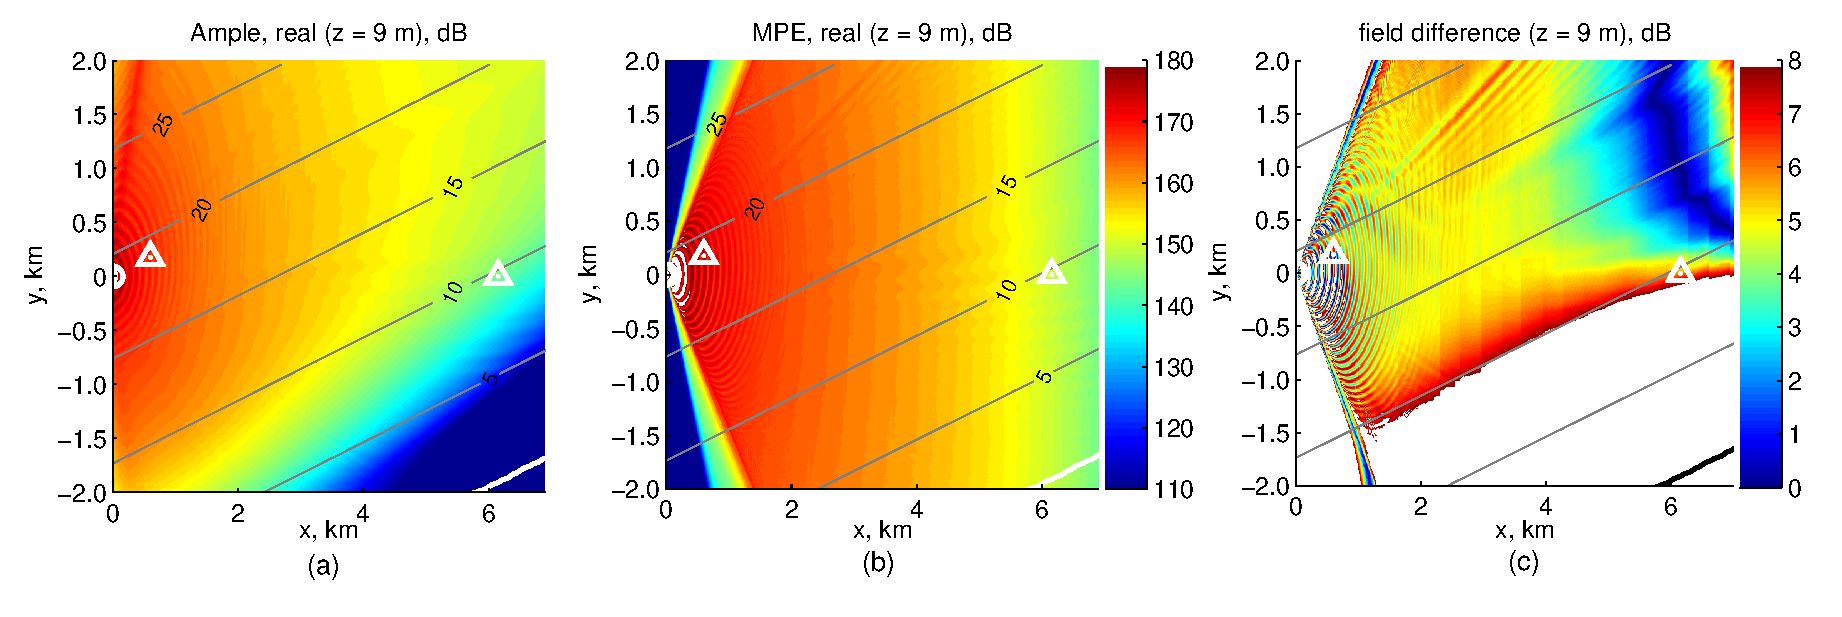
\includegraphics[width=0.9\textwidth]{images/seismo/pic_lineField.eps}
                        \caption{Пространственное распределение уровня звуковой экспозиции при глубине 9 м, вычисленное с использованием AMPLE (\textbf{a}) и MPE(\textbf{b}) для моделирования распространения в волноводе с донным наклоном, заданным уравнением \ref{m_polynom}. Абсолютная разница между ними также отражена на (\textbf{c}).}
                        \label{fig4:scheme}
                    \end{figure}

                    \FloatBarrier

            \subsubsection{Результаты моделирования с учётом реальной батиметрии}
                \par Далее рассматривается точность вычисления уровней звуковой экспозиции, с использованием программ AMPLE и MPE, на примере волновода с реалистичной батиметрией. В данном случае моделируется форма сигнала в точке P2 и оценивается точность моделей прямым сравнением с данными измерений.

                \par На Рис. \ref{fig5:SEL} -- \ref{fig7:waveform_and_spectra} отображены результаты вычислений. Контурные графики на Рис. \ref{fig5:SEL} показывают, что структура распределения уровня звуковой экспозиции в данном случае является качественно схожей с таковыми, полученными для упрощённой модели батиметрии \eqref{m_polynom}. Стоит заметить, что абсолютная разница между результатами вычислений моделей (см. Рис. \ref{fig5:SEL}c) в данном случае также схоже с Рис. \ref{fig4:scheme}c. Распределения звуковой экспозиции явно отражают батиметрию в рассматриваемой области, и их структура также показывает проявление типичных эффектов горизонтальной рефракции в волноводах мелкого моря (большая амплитуда поля в областях с большей глубиной).

                \begin{figure}[h]
                    \centering
                    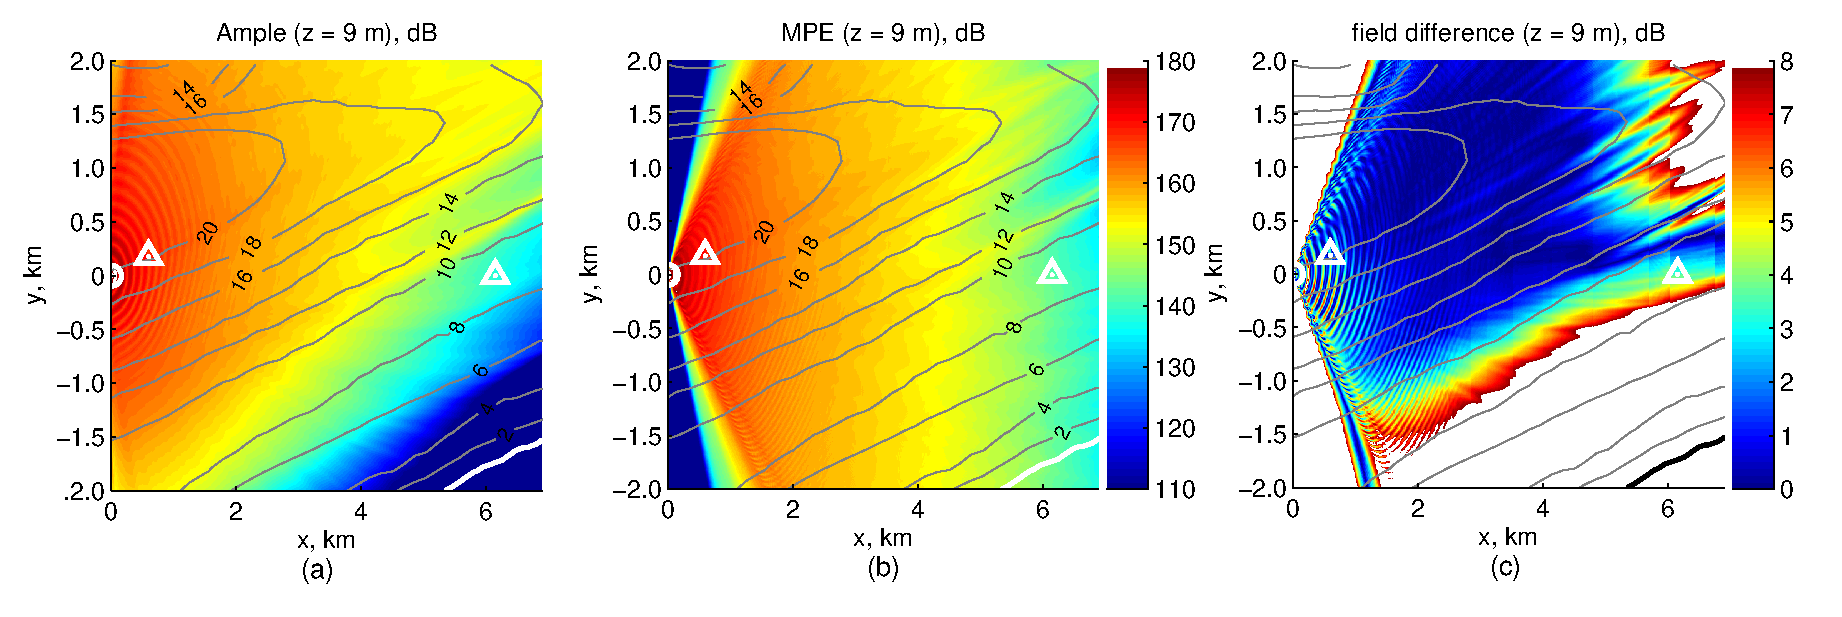
\includegraphics[width=0.9\textwidth]{images/seismo/pic_realField.eps}
                    \caption{Пространственное распределение значения звуковой экспозиции на глубине 9 м, вычисленное с использованием AMPLE (\textbf{a}) и MPE(\textbf{b}) для волновода с реалистичной батиметрией. Абсолютная разница между ними также отражена на (\textbf{c}).}
                    \label{fig5:SEL}
                \end{figure}

                \par Стоит также заметить, что результаты, полученные с использованием AMPLE и MPE, показывают хорошее согласие по направлению распространения (то есть по прямой $y=0$, см. Рис. \ref{fig6:SEL}). Однако, при удалении от этой прямой возникает существенное различие между предсказаниями моделей (см. Рис. \ref{fig5:SEL}c). Ясно, что разница возникает из ограниченной апертуры в горизонтальной плоскости в модели, используемой в MPE. Важно отметить, что различие достигает 8 дБ даже при отклонении от оси распространения на $\pm3.5^\circ$ на расстоянии около $7$ км от источника.

                \par На Рис. \ref{fig6:SEL} также приведено сравнение форм сигнала, вычисленных моделями в точке P2 (при расчётах спектр источника был восстановлен на основе сигнала в точке P1). Как видно из рисунка, сигнал, полученный с использованием AMPLE, показывает существенно большее качественное и количественное сходство с данными измерений.

                \begin{figure}[h]
                    \centering
                    \includegraphics[width=0.9\textwidth]{images/seismo/pic_test_sel.eps}
                    \caption{График зависимости уровня звуковой экспозиции от расстояния $x$ на прямой $y=0$ и глубине 9 м, вычисленной с использованием AMPLE и MPE для упрошённой и реальной батиметрии.}
                    \label{fig6:SEL}
                \end{figure}

                \begin{figure}[h]
                    \centering
                    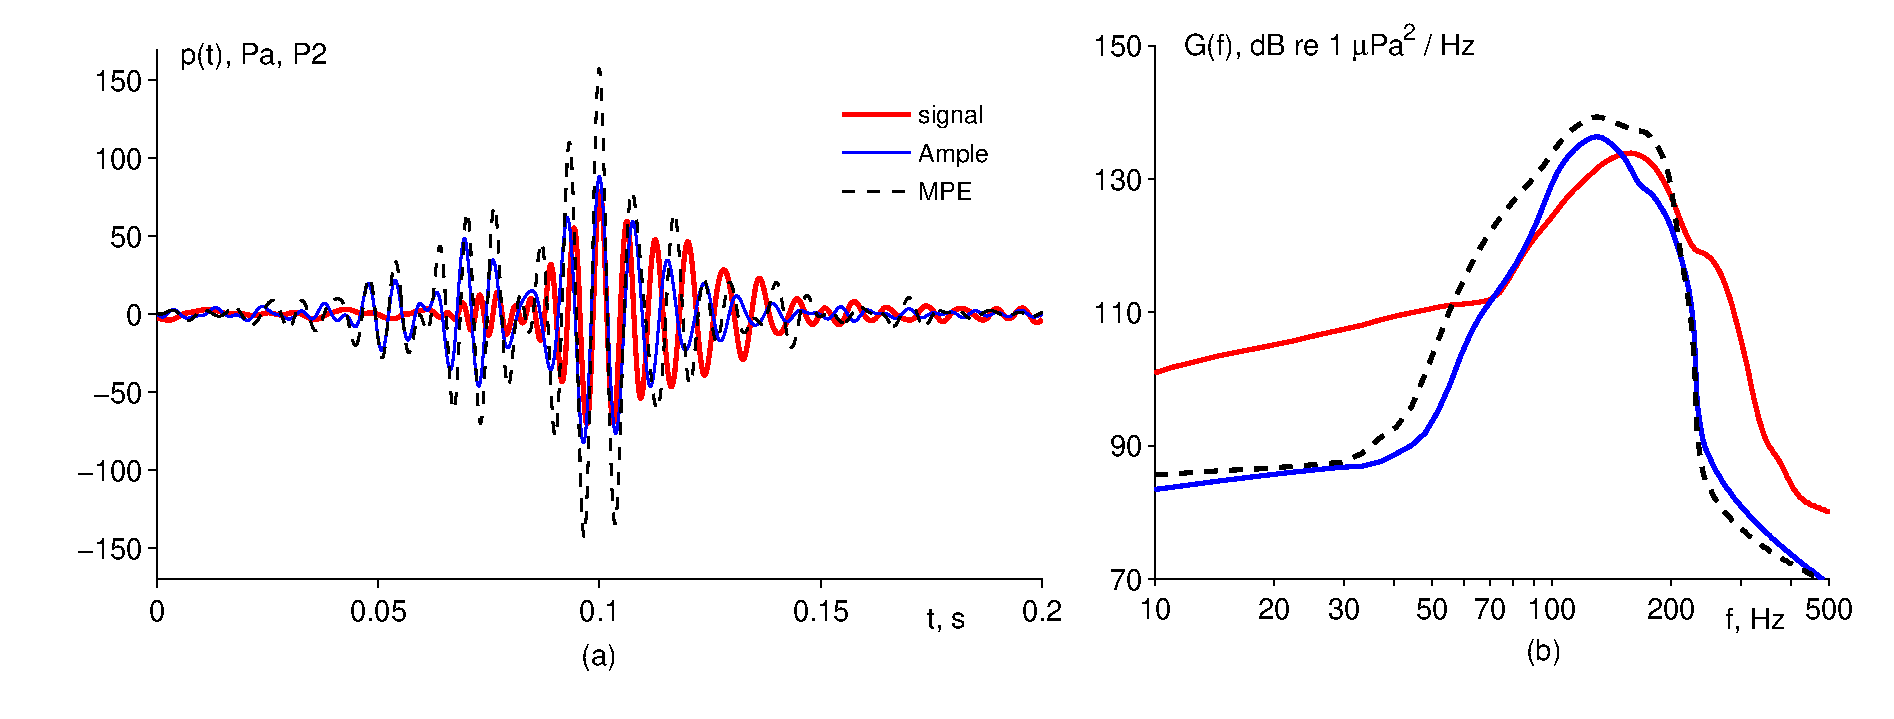
\includegraphics[width=0.9\textwidth]{images/seismo/pic_signal3.eps}
                    \caption{Сравнение импульсных сигналов (\textbf{a}) и их спектров (\textbf{b}), полученные из данных измерений и результатов моделирования в точке P2.}
                    \label{fig7:waveform_and_spectra}
                \end{figure}

                \FloatBarrier

        \subsection{Выводы к четвёртой главе}
            \par В данной главе диссертации рассмотрено моделирование широкополосных звуковых полей в двух случаях: шумы, наблюдаемые при движении морского судна, а также шумы, связанные с проведением сейсморазведки. Такое моделирование имеет огромное значение для проведения оценки антропогенных шумов в областях, для которых прямые измерения не могут быть проведены с необходимым пространственным разрешением для оценки их влияния на окружающую среду. Выполнение такого рода оценок составляет задачу акустического мониторинга, имеющую целью защиту различных видов морских животных от шумового воздействия.

            \par В случае моделирования шума одиночного судна точное предсказание уровней звукового поля потребовало адекватной оценки параметров среды. Действительно, оптимизация показала, что предсказания звукового поля были особенно чувствительны к контрасту геоакустических параметров на границе раздела вода-дно. Грубая оценка, основанная на геологических картах и таблицах типичных геоакустических свойств различных видов твёрдых пород и осадков, может быть недостаточной для данной задачи. Вместо этого стоит провести геоакустическую инверсию (или, широко говоря, оптимизацию параметров), используя подходящие источники или проводя специализированные эксперименты по измерению потерь на распространение. Некоторые подходы к оценке геоакустических параметров дна известны в литературе, например  \cite{gervaise2012,knobles2015, tollefsen2021}. В рамках данной задачи, использование параметров, оптимизированных с учетом измерений в единственной точке (а именно точки ближайшего прохода), позволило существенно улучшить точность предсказания уровней шумов на всей акватории.

            \par Важно обратить внимание, что оптимизированные значения параметров среды с высокой долей вероятности будут в некотором смысле нефизическими и позволяют лишь параметризовать настоящее дно таким образом, чтобы потери на распространение были приведены в соответствие результатам натурных измерений (например, большое значение параметра затухания компенсирует отсутствие поперечных волн в использованной модели, что в контексте рассматриваемой задачи может быть рассмотрено как механизм возникновения дополнительных потерь). Стоит упомянуть, что использование среднемноголетних данных о профиле скорости звука также может привести к ошибкам в предсказании уровней шума. Лучшим вариантом может быть использование профилей скорости звука, полученных с использованием моделей циркуляции океана, особенно в тех областях, где такие модели ассимилируют местные измерения.

            \par Данная глава также демонстрирует важность учёта трёхмерных эффектов распространения звука при проведении моделирования акустического поля. Однако необходимо отметить, что использование трёхмерны моделей, требующих проведения существенно больших вычислений по сравнению с их вдумерынми аналогами, имеет смысл лишь после проведения оптимизации параметров дна, так как в обратном случае гораздо более значительные ошибки будут возникать из-за неточности информации о самих параметрах среды.

            \par Конечно вероятно, что такое большое судно не может быть точно представлено в виде точечного источника, и вид его направленности должен быть учтён \cite{cybulski1977probable,gassman2017}, так как иначе даже параметры, оптимизированные относительно точки ближайшего прохода, не могут гарантировать идеальное представление звукового поля для большого интервала частот (например, EC2). Действительно, размеры сухогруза в рассматриваемом сценарии сравнимы с его расстоянием ближайшего прохода от гидрофона. Наличие данных измерений, содержащих информацию об изменениях фазы (а не только амплитуды) может позволить рассмотреть параметризацию источника множеством точечных источников, спектр которых наверное может быть оценен. Представление судов в виде пространственно распределённых источников шума при проведении измерений подводными акустическими станциями является предметом текущих исследований \cite{echo2021}.

            \par В случае моделирование распространения шума, возникающего в результате проведения сейсмологической разведки, было проведено моделирование уровня звуковой экспозиции в большой морской области. При этой результаты измерений в опорной точке были использованы для восстановления эффективного спектра источника, который затем использован для вычисления поля уровня звуковой экспозиции во всей акватории рассматриваемой области.

            \par При проведении моделирования были использованы данные, полученные во время проведения сейсмологической разведки в Охотском море на Сахалинском шельфе. Сейсмический импульс, создаваемый разведовательным судном, был записан в двух точках. Результаты измерений, полученные в точке P1 на расстоянии около 600 м от источника S, были использованы для восстановления спектра источника, в то время как данные, полученные в точке P2, были использованы для оценки результатов моделирования.

            \par Было показано, что решение модовых параболических уравнений позволяет восстановить форму сигнала в точке P2 с удовлетворительной точностью, как во временной, так и в частотной областях. Также важно отметить, что использование широкогольных модовых параболических уравнений позволяет достичь существенно большей точности предсказания, по сравнению с их узкогольными аналогами, учитывающими взаимодействие мод. Несмотря на то, что значение звуковой экспозиции воспроизводится моделями с достаточной точностью для использования в прикладных задачах, наблюдается существенная разница спектров в частотном диапазоне 10-50 Герц (как видно на Рис. \ref{fig7:waveform_and_spectra}). Как и в случае моделирования шума единственного судна, такое различие можно объяснить недостаточно точной моделью морского дна, поэтому точность предсказания моделей также может быть повышена использованием геокустической инверсии для восстановления структуры и параметров дна напрямую из данных измерений. В случае с распространением сейсморазведовательных импульсов такая инверсия может быть выполнена с использованием моделей, основанных на свертках \cite{bonnel2020}. Использование такого подхода также может способствовать дальнейшему увеличению точности предсказания уровня звуковой экспозиции. Конечно, даже в таком идеальном случае, полученные параметра дна представляли бы собой лишь грубую аппроксимацию морской среды, что все равно может привести к пренебрежению важными трёхмерными эффектов вдоль и поперёк направления распространения звука \cite{lunkov2021}.
            \par Результаты второй главы опубликованы в работах \cite{jmse,petrov2024_2}.
\end{document}
